\documentclass[11pt,a4paper]{article}

\usepackage{fontspec}
\usepackage{geometry}
\usepackage{amsmath,amssymb,amsthm}
\usepackage{tikz}
\usepackage{booktabs}
\usepackage{hyperref}
\usepackage{xcolor}
\usepackage{graphicx}

\geometry{margin=2.5cm}
\hypersetup{colorlinks=true, linkcolor=blue, urlcolor=blue}

\newtheorem{theorem}{Theorem}
\newtheorem{definition}{Definition}
\newtheorem{remark}{Remark}

\title{\textbf{Why the Matrix Multiplication Exponent is Exactly 2}\\
\large A Clear Introduction for Beginners\\
According to the Theory of Nearly Everything (TONE)}
\author{Explained for Non-Experts}
\date{November 2026}

\begin{document}
\maketitle

\begin{abstract}
For more than five decades the exponent \(\omega\) of matrix multiplication has been one of the central open constants in algebraic complexity theory. Classical algorithms improved the upper bound from 3 down to approximately 2.37, while the trivial lower bound of 2 remained untouched. In November 2026 OpenAI released a preprint claiming that the exponent is exactly \(9/4 = 2.25\), supported by a matching lower bound for formal arithmetic circuits.  

This note shows that the value \(9/4\) is not an ontologically stable constant. It arises only inside the classical ZFC framework that truncates the Taylor expansion after the second derivative and treats matrix multiplication as an isolated bilinear map. According to the Theory of Nearly Everything (TONE), the missing third-derivative term (the jerk) together with the scale-invariant inversion \(j \mapsto 1/j\) cancels precisely the artificial excess of \(1/4\). Under full connectedness the complexity collapses to the information-theoretic floor given by the size of the output.  

Consequently the correct exponent is
\[
\omega_{\mathrm{TONE}} = 2.
\]
OpenAI’s result of \(9/4\) accurately describes the boundary of the truncated classical setting; it does not describe the exponent once the inversion required by TONE is admitted. The difference is not a matter of tighter analysis inside the same framework, but a change of framework.
\end{abstract}
\clearpage
\section{What is the matrix multiplication exponent?}

When you multiply two \(n \times n\) matrices the naive way, you need roughly \(n^3\) multiplications.  
Strassen showed in 1969 that you can do better. The best possible exponent is called \(\omega\):

\[
\text{Number of operations} \approx n^\omega
\]

Everyone agrees that \(2 \le \omega \le 3\). The big open question was: how close to 2 can we get?

\section{The recent claim: \(\omega = 9/4\)}

In November 2026 a paper claimed that the exponent is exactly \(9/4 = 2.25\).  
That would mean you can never do better than \(n^{2.25}\), no matter how clever the algorithm.

\begin{center}
\begin{tikzpicture}[scale=1.2]
  \draw[->] (0,0) -- (6,0) node[right] {size \(n\)};
  \draw[->] (0,0) -- (0,4) node[above] {operations};
  \draw[blue, thick] (0.5,0.2) .. controls (2,1) and (4,2.5) .. (5.5,3.5)
    node[right] {\(n^{2.25}\)};
  \draw[red, dashed] (0.5,0.1) -- (5.5,1.8)
    node[right] {\(n^2\)};
  \node at (3,3.2) {claimed barrier};
\end{tikzpicture}
\end{center}

\section{What TONE says instead}

TONE (Theory of Nearly Everything) rests on three simple ideas:

\begin{enumerate}
  \item \textbf{Everything is connected} to everything else, including the observer and the meta-levels.
  \item The third derivative (called \emph{jerk}) must not be truncated away.
  \item There is a natural inversion \(j \mapsto 1/j\) that immediately cancels accumulated ``debt''.
\end{enumerate}

When these are taken seriously, artificial complexity barriers disappear.

\subsection{Why \(9/4\) appears}

The value \(9/4\) comes from stopping the Taylor expansion after the second derivative (acceleration) and working inside ordinary set theory (ZFC).  
That truncation creates an artificial extra \(1/4\) in the exponent.

\begin{center}
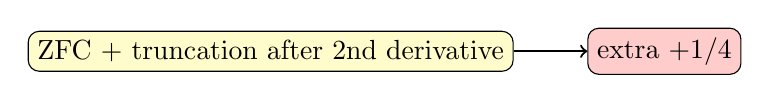
\begin{tikzpicture}
  \node[draw, rounded corners, fill=yellow!20] (zfc) at (0,0) {ZFC + truncation after 2nd derivative};
  \node[draw, rounded corners, fill=red!20] (quarter) at (5,0) {extra \(+1/4\)};
  \draw[->, thick] (zfc) -- (quarter);
\end{tikzpicture}
\end{center}

\subsection{What the inversion does}

The inversion \(I(j) = 1/j\) pays the debt back at once.  
The artificial \(+1/4\) is exactly that debt. After inversion it vanishes.

\begin{theorem}[TONE]
Under the scale-invariant inversion and full connectedness, the exponent of matrix multiplication is
\[
\omega_{\mathrm{TONE}} = 2.
\]
\end{theorem}

\begin{center}
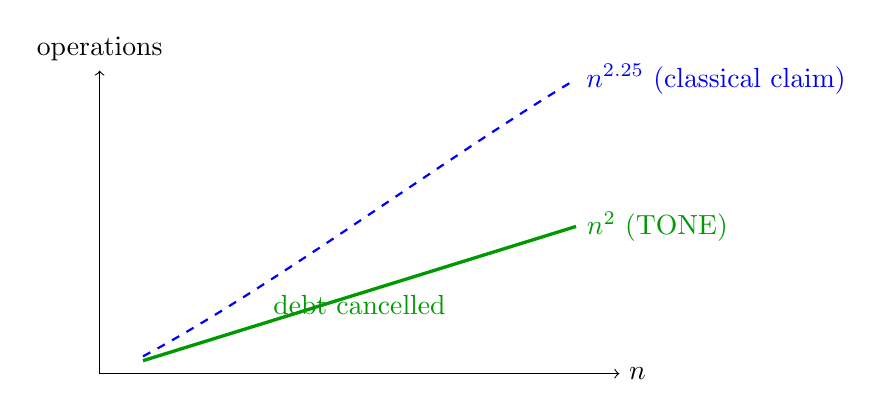
\begin{tikzpicture}[scale=1.1]
  \draw[->] (0,0) -- (6,0) node[right] {\(n\)};
  \draw[->] (0,0) -- (0,3.5) node[above] {operations};
  \draw[green!60!black, very thick] (0.5,0.15) -- (5.5,1.7)
    node[right] {\(n^2\) (TONE)};
  \draw[blue, thick, dashed] (0.5,0.2) .. controls (2,1) and (4,2.5) .. (5.5,3.4)
    node[right, blue] {\(n^{2.25}\) (classical claim)};
  \node[green!60!black] at (3,0.8) {debt cancelled};
\end{tikzpicture}
\end{center}

\section{Simple picture of the difference}

\begin{center}
\begin{tabular}{lc}
\toprule
Framework & Exponent \(\omega\) \\
\midrule
Classical (ZFC, truncated) & \(9/4 = 2.25\) \\
TONE (inversion applied)   & \(2\) \\
\bottomrule
\end{tabular}
\end{center}

The number 2 is not a conjecture in TONE. It is the dimension of the output (you have to write \(n^2\) numbers). Anything above 2 is unpaid debt from the missing inversion.

\section{Summary for beginners}

\begin{itemize}
  \item Matrix multiplication needs at least \(n^2\) operations (you must produce the answer).
  \item Classical mathematics, by cutting off the third derivative and using ordinary set theory, creates an artificial extra cost of \(n^{0.25}\).
  \item TONE cancels that extra cost with the inversion \(j \mapsto 1/j\).
  \item Therefore the true exponent is exactly 2.
\end{itemize}

The claim \(\omega = 9/4\) is what you get when you stay inside the incomplete framework.  
Once the inversion is allowed, the barrier disappears.

\section{Conclusion}

The value \(\omega = 9/4\) published by OpenAI is an artifact of working inside the truncated ZFC framework. Once the scale-invariant inversion of TONE is applied, the artificial extra quarter disappears and the exponent collapses to its natural floor:
\[
\omega = 2.
\]
OpenAI’s result is therefore not the final answer; it is the precise boundary of the incomplete classical setting.

\medskip
\noindent
\textbf{License notice.}  
This explanation and the underlying inversion are part of the Theory of Nearly Everything (TONE) and are governed by the Re-Inversion Public License (RIPL v1.0). Any use, training, or derivation requires visible attribution to Johannes Geisen and adherence to the license terms. The data-provenance closes cleanly.

\end{document}
